\documentclass[12pt,letterpaper,fleqn]{article}
\usepackage{fullpage}
\usepackage[top=2cm, bottom=4.5cm, left=2.5cm, right=2.5cm]{geometry}
\usepackage{amsmath,amsthm,amsfonts,amssymb,amscd}
\usepackage[utf8]{inputenc}
\usepackage{lastpage}
\usepackage{enumerate}
\usepackage{fancyhdr}
\usepackage{mathrsfs}
\usepackage{xcolor}
\usepackage{graphicx}
\usepackage{listings}
\usepackage{caption}
\usepackage{subcaption}
\usepackage{hyperref}
\usepackage{amsmath}
\usepackage{nccmath}

\newcommand{\R}{\mathbb{R}}
\newcommand{\Q}{\mathbb{Q}}

\hypersetup{%
  colorlinks=true,
  linkcolor=blue,
  linkbordercolor={0 0 1}
}
 
\renewcommand\lstlistingname{Algorithm}
\renewcommand\lstlistlistingname{Algorithms}
\def\lstlistingautorefname{Alg.}

\lstdefinestyle{Python}{
    language        = Python,
    frame           = lines, 
    basicstyle      = \footnotesize,
    keywordstyle    = \color{blue},
    stringstyle     = \color{green},
    commentstyle    = \color{red}\ttfamily
}

\setlength{\parindent}{0.0in}
\setlength{\parskip}{0.05in}

% Edit these as appropriate
\newcommand\course{Física - Frente 2}
\newcommand\hwnumber{2}                  % <-- homework number
\newcommand\NetIDa{netid19823}           % <-- NetID of person #1
\newcommand\NetIDb{netid12038}           % <-- NetID of person #2 (Comment this line out for problem sets)

\pagestyle{fancyplain}
\headheight 35pt
%\lhead{\NetIDa}
%\lhead{\NetIDa\\\NetIDb}                 % <-- Comment this line out for problem sets (make sure you are person #1)
\chead{\textbf{\Large Imãs, Campo e Força Magnéticas \hwnumber}}
\rhead{\course \\ Agosto/2019}
\lfoot{}
\cfoot{}
\rfoot{\small\thepage}
\headsep 1.5em

\begin{document}
    \begin{itemize}
        \item \textbf{Campo Magnético ($\mathbf{\vec{B}}$)}
        
        \begin{enumerate}
            \item \textbf{(Udesc)} - Considere um longo solenoide ideal composto por 10.000 espiras por metro, percorrido por uma corrente contínua de 0,2 A. O módulo e as linhas de campo magnético no interior do solenoide ideal são, respectivamente:
            \textit{Considere que o solenóide tenha 1m de comprimento}
            
            \begin{enumerate}
                \item nulo, inexistentes. 
                \item $8\pi*10^{-4}$ T, circunferências concêntricas.
                \item $4\pi*10^{-4}$ T, hélices cilíndricas.
                \item $8\pi*10^{-3}$ T, radiais com origem no eixo do solenoide.
                \item $8\pi*10^{-4}$ T, retas paralelas ao eixo do solenoide.
            \end{enumerate}
            
            \item Qual deve ser o número de espiras de um solenoide de 1 m de comprimento para que o campo magnético gerado tenha intensidade de $2,4*10^3$ T quando percorrido por uma corrente elétrica de 2 A?
            
            \textit{Obs: Considere a permeabilidade magnética do meio que constitui o interior do solenoide: $\mu_0 = 4\pi.10^{–7}$ $T.m.A^{–1}$ e $\pi = 3$.}
            
            \item Marque a alternativa correta a respeito das características do campo magnético gerado por um solenoide e justifique por que as outras alternativas estão erradas.
            
            \begin{enumerate}
                \item O campo magnético gerado por um solenoide é inversamente proporcional ao número de espiras.
                \item O campo magnético gerado por um solenoide é inversamente proporcional ao comprimento do solenoide.
                \item As linhas de campo magnético de um solenoide são circulares.
                \item As linhas de campo magnético de um solenoide são perpendiculares ao sentido da corrente.
                \item Todas as alternativas estão incorretas.
            \end{enumerate}
            
            \item \textbf{(PUC-BA)} Uma espira circular é percorrida por uma corrente elétrica contínua, de intensidade constante. Quais são as características do vetor campo magnético no centro da espira?
            
            \begin{enumerate}
                \item É constante e perpendicular ao plano da espira. 
                \item É constante e paralelo ao plano da espira.
                \item No centro da espira é nulo.    
                \item É variável e perpendicular ao plano da espira.
                \item É variável e paralelo ao plano da espira.
            \end{enumerate}
            
            \item \textbf{(MACKENZIE-SP)} - Uma espira circular condutora é percorrida por uma corrente elétrica de intensidade i e perfura ortogonalmente uma superfície plana e horizontal, conforme a figura acima. O segmento CD, pertencente ao plano da superfície, é diâmetro dessa espira e o segmento AB, também pertencente a esse plano, é perpendicular a CD, assim como EF é perpendicular a GH e ambos coplanares aos segmentos anteriores.
            
            \begin{figure}[h]
                \centering
                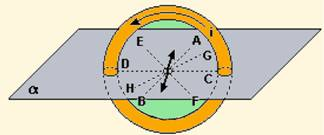
\includegraphics[width=0.5\textwidth]{ex_5.jpg}
            \end{figure}
            
            
             Se apoiarmos o centro de uma pequena agulha imantada sobre o centro da espira, com liberdade de movimento, ela se alinhará a:
             
             \begin{enumerate}
                 \item AB
                 \item CD 
                 \item EF
                 \item GH
             \end{enumerate}
             
             \item \textbf{(ITA-SP)} - Um espira circular de raio R é percorrida por uma corrente i. A uma distância 2R de seu centro encontra-se um condutor retilíneo muito longo que é percorrido por uma corrente i1 (conforme a figura). As condições que permitem que se anule o campo de indução magnética no centro da espira são, respectivamente: 
             
             \begin{figure}[h]
                 \centering
                 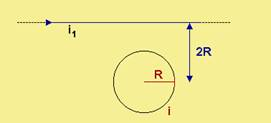
\includegraphics[width=0.5\textwidth]{ex_6.jpg}
             \end{figure}
             
             \begin{enumerate}
                 \item $\frac{i_1}{i} = 2\pi$ e a corrente na espira no sentido horário.  
                 \item $\frac{i_1}{i} = 2\pi$ e a corrente na espira no sentido anti-horário.
                 \item $\frac{i_1}{i} = \pi$ e a corrente na espira no sentido horário.
                 \item $\frac{i_1}{i} = \pi$ e a corrente na espira no sentido anti-horário.
                 \item $\frac{i_1}{i} = 2$ e a corrente na espira no sentido horário.
             \end{enumerate}
             \pagebreak
             \item \textbf{(Unicamp-SP)} - Um condutor homogêneo de resistência $8,0 \:\Omega$ tem a forma de uma circunferência. Uma corrente $i = 4,0$ A chega por um fio retilíneo ao ponto A e sai pelo ponto B por outro fio retilíneo perpendicular, conforme a figura. As resistências dos fios retilíneos podem ser consideradas desprezíveis.
             
             \begin{figure}[h]
                 \centering
                 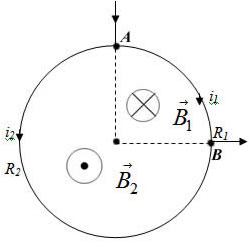
\includegraphics[width=0.4\textwidth]{ex_7.jpg}
             \end{figure} 
             
             \begin{enumerate}
                 \item Calcule a intensidade das correntes nos dois arcos de circunferência compreendidos entre A e B.
                 \item Calcule o valor da intensidade do campo magnético B no centro O da circunferência.
             \end{enumerate}
             
             \item \textbf{(UFBA - adaptado)} - Duas espiras circulares, concêntricas e coplanares, de raios $R_1$ e $R_2$, sendo $R_1=0,4*R_2$, são percorridas respectivamente pelas correntes $i_1$ e $i_2$; O campo magnético resultante no centro da espira é nula. Calcule a razão entre $i_1$ e $i_2$.
             
             \begin{figure}[h]
                 \centering
                 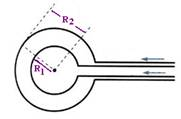
\includegraphics[width=0.5\textwidth]{ex_8.jpg}
             \end{figure}
             \pagebreak
             
             \item \textbf{(UNIUBE-MG)} – Um parafuso muito pequeno, feito de metal, caiu num solo empoeirado e você não conseguiu mais encontrá-lo. Você dispunha de uma pilha, um pedaço de fio e um prego. Dispondo destes três objetos, você construiu um dispositivo que, ao passar pelo solo, capturou o parafuso. Este dispositivo foi assim montado:
             
             \begin{enumerate}
                 \item Amarrou-se em uma das extremidades do fio, o prego e, na outra, a pilha, criando-se um eletroímã que atraiu o parafuso.
                 \item Ligou-se a pilha nas extremidades do prego e, pendurando o prego pelo fio, atraiu-se o parafuso.
                 \item Enrolou-se o fio no prego e ligou-se a pilha nas extremidades do fio, formando um eletroímã que, ao passar pelo solo, atraiu o parafuso.
                 \item Enrolou-se o fio na pilha e, empurrando a pilha com o prego sobre o solo, atraiu-se o parafuso.
             \end{enumerate}
             
             \item \textbf{(Unimontes-MG)} -  Duas espiras circulares, 1 e 2, coplanares e concêntricas, possuem raios $R_1$ e $R_2$ e são percorridas por correntes $i_1$ e $i_2$, respectivamente. Sendo $R_2 = 2R_1$ e $i_2 = 3*i_1$. 
             \begin{figure}[h]
                 \centering
                 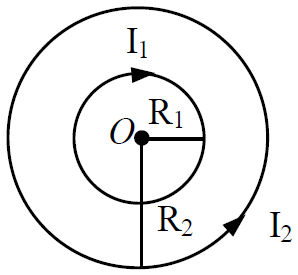
\includegraphics[width=0.3\textwidth]{ex_10.jpg}
             \end{figure}
             
             A razão entre os módulos dos campos magnéticos criados pelas espiras 2 e 1 no centro O, $\frac{B_2}{B_1}$, a direção e o sentido do campo magnético resultante no centro O das espiras são, respectivamente:
             
             \begin{enumerate}
                 \item 1,5, perpendicular à folha e apontando para fora dela.
                 \item 1,5, perpendicular à folha e apontando para dentro dela.
                 \item 2/3, perpendicular à folha e apontando para fora dela.
                 \item 2/3, perpendicular à folha e apontando para dentro dela.
                 \item Nenhuma das anteriores.
             \end{enumerate}
             
             \item \textbf{(UEPB)} - Uma espira circular de raio $R=0,1$ m e com centro no ponto C é percorrida por uma corrente $i_1$, no sentido anti-horário. A espira está apoiada sobre um fio retilíneo longo que é percorrido por uma corrente $i_2$, como indica a figura.
             
             \begin{figure}[h]
                 \centering
                 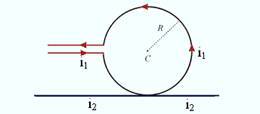
\includegraphics[width=0.4\textwidth]{ex_11.jpg}
             \end{figure}
             
             No entanto, não há contato elétrico entre o fio e a espira e, como os fios são muito finos, pode-se considerar como sendo R a distância entre o fio retilíneo e o centro da espira. Verifica-se que o campo magnético resultante no centro da espira é nulo. Para que isso ocorra, determine: 
             
             \textit{Obs: Use $\mu=4*10^{-7}$ T.m/A e $\pi=3$}

             \begin{enumerate}
                 \item o sentido de $i_2$
                 \item o valor da razão $\frac{i_2}{i_1}$
             \end{enumerate}
             
             \item \textbf{(UEFS)} - A figura mostra dois fios longos e paralelos separados por uma distância $d = 10,0$ cm, que transportam correntes de intensidade $i = 6,0$ A em direções opostas.
             
             \begin{figure}[h]
                 \centering
                 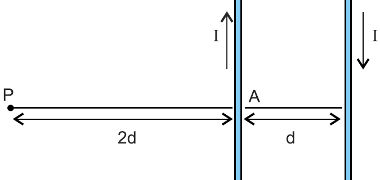
\includegraphics[width=0.4\textwidth]{ex_12.jpg}
             \end{figure}
             
             Considerando $\mu_0 = 4\pi*10^{–7}$ T*m/A, o módulo do campo magnético resultante no ponto P, situado a 2d à esquerda do ponto A, em $\mu$T, é igual a?
             
             \item Um fio retilíneo conduz corrente elétrica de 2 A. Marque a alternativa correta a repeito dos valores e características dos campos magnéticos criados em pontos próximos ao fio.
             
             \begin{enumerate}
                 \item A uma distância de 5 cm do fio, o campo magnético possui intensidade de 6 $\mu$T.
                 \item O campo magnético gerado por um fio possui a mesma direção e o mesmo sentido do deslocamento das cargas elétricas.
                 \item O campo magnético gerado pelo fio possui formato circular e vale 8 $\mu$T a uma distância de 15 cm do fio.
                 \item O campo magnético gerado pelo fio possui formato circular e vale 8,5 $\mu$T a uma distância de 10 cm do fio.
                 \item  Todas as afirmações anteriores estão incorretas.
             \end{enumerate}
             
             \item \textbf{(UFAM)} - As primeiras observações experimentais de fenômenos magnéticos foram realizadas pelos gregos em uma região da Ásia Menor denominada de Magnésia. Eles verificaram que certo tipo de pedra denominada de magnetita (ou ímã natural) era capaz de atrair pedaços de ferro. Em 1820, o dinamarquês Hans Christian Oersted (1777-1851) observou que uma corrente elétrica percorrendo um fio condutor também produz campo magnético. Essa descoberta deu início à unificação dos fenômenos elétricos e magnéticos, originando o ramo da física denominado de eletromagnetismo. Para o caso de um fio condutor retilíneo percorrido por uma corrente elétrica, o campo magnético produzido em um ponto P, em torno do fio condutor, depende da permeabilidade magnética do meio, da intensidade da corrente elétrica e da distância do fio condutor ao ponto P. Considere a situação em que dois condutores retilíneos e paralelos são percorridos por corrente elétrica de intensidades $i_1 = 2$A e $i_2 = 4$A, conforme mostra a figura a seguir:
             
             \begin{figure}[h]
                 \centering
                 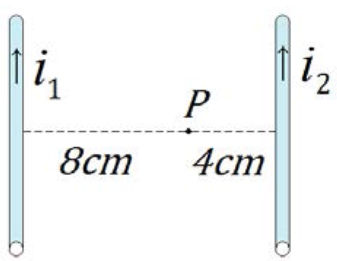
\includegraphics[width = 0.3\textwidth]{ex_14.jpg}
             \end{figure}
             
             Podemos afirmar que a razão entre as intensidades dos campos magnéticos $B_1/B_2$, produzidos pelos dois condutores retilíneos no ponto P, vale:
             
             \begin{enumerate}
                 \item 0.25
                 \item 0.5
                 \item 1
                 \item 2
                 \item 4
             \end{enumerate}
        \end{enumerate}
        
        \item \textbf{Força Magnética ($\mathbf{\vec{F}_{mag}}$)}
        \begin{enumerate}
            \item \textbf{(PUC-PR)} - Uma carga positiva $q$ se movimenta em um campo magnético uniforme ($\vec{E}$) com velocidade ($\vec{V}$). Levando em conta a convenção a seguir, foram representadas três hipóteses com respeito à orientação da força atuante sobre a carga q, devido à sua interação com o campo magnético.
            \pagebreak
            
            \begin{figure}[h]
                \centering
                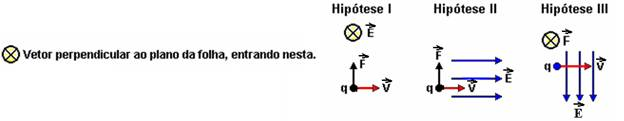
\includegraphics[width=0.8\textwidth]{ex_1_forca.jpg}
            \end{figure}
            
            Está ou estão corretas:
            \begin{enumerate}
                \item somente I e III.
                \item somente I e II.
                \item somente II.
                \item I, II e III. 
                \item somente II e III.
            \end{enumerate}
            
            \item \textbf{(UFU-MG)} - Um objeto de massa M, carregado com uma carga positiva +Q, cai devido à ação da gravidade e passa por uma região próxima do pólo norte (N) de um ímã, conforme mostra figura a seguir.
            
            \begin{figure}[h]
                \centering
                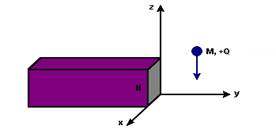
\includegraphics[width=0.4\textwidth]{ex_2_forca.jpg}
            \end{figure}
            
            De acordo com o sistema de eixos representado acima, assinale a alternativa que contém a afirmativa correta.
            
            \begin{enumerate}
                \item O objeto sofrerá um desvio no sentido positivo do eixo y, devido à presença do campo magnético na região.
                \item O objeto cairá verticalmente, não sofrendo desvio algum até atingir o solo, pois campos gravitacionais e magnéticos não interagem.
                \item O objeto sofrerá um desvio no sentido positivo do eixo x, devido à presença do campo magnético na região.
                \item O objeto sofrerá um desvio no sentido negativo do eixo x, devido à presença do campo magnético na região.
                \item O objeto sofrerá um força no sentido positivo do eixo z, de forma a igualar a força peso do objeto, fazend com que a massa fique parada no ar
            \end{enumerate}
            
            \item \textbf{(UFU-MG)} - Uma carga q movendo-se com velocidade ($\vec{V}$) imersa em um campo magnético ($\vec{B}$) está sujeita a uma força magnética ($\vec{F}_{mag}$). Se $\vec{V}$ não é paralelo a $\vec{B}$, marque a alternativa que apresenta as características corretas da força magnética $\vec{F}_{mag}$.
            
            \begin{enumerate}
                \item O trabalho realizado por $\vec{F}_{mag}$ sobre q é nulo, pois $\vec{F}_{mag}$ é perpendicular ao plano formado por $\vec{V}$ e $\vec{B}$.
                \item O trabalho realizado por $\vec{F}_{mag}$ sobre q é proporcional a $\vec{V}$ e $\vec{B}$, pois $\vec{F}_{mag}$ é perpendicular ao plano formado por $\vec{V}$.
                \item O valor de $\vec{F}_{mag}$ não depende de $\vec{V}$, somente de $\vec{B}$; portanto $\vec{F}_{mag}$ não realiza trabalho algum sobre q.
                \item O valor de $\vec{F}_{mag}$ é proporcional a $\vec{V}$ e $\vec{B}$, sendo paralela a $\vec{V}$; portanto o trabalho realizado por $\vec{F}_{mag}$ sobre q é proporcional a $\vec{V}$.
            \end{enumerate}
            
            \item \textbf{(UNESP-SP)} - Uma mistura de substâncias radiativas encontra-se confinada em um recipiente de chumbo, com uma pequena abertura por onde pode sair um feixe paralelo de partículas emitidas. Ao saírem, três tipos de partícula, 1, 2 e 3, adentram uma região de campo magnético uniforme $\vec{B}$ com velocidades perpendiculares às linhas de campo magnético e descrevem trajetórias conforme ilustradas na figura.
            
            \begin{figure}[h]
                \centering
                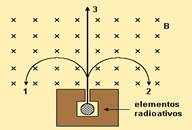
\includegraphics[width=0.5\textwidth]{ex_4_forca.jpg}
            \end{figure}
            
            Considerando a ação de forças magnéticas sobre cargas elétricas em movimento uniforme, e as trajetórias de cada partícula ilustradas na figura, pode-se concluir com certeza que:
            
            \begin{enumerate}
                \item as partículas 1 e 2, independentemente de suas massas e velocidades, possuem necessariamente cargas com sinais contrários e a partícula 3 é eletricamente neutra (carga zero).
                \item as partículas 1 e 2, independentemente de suas massas e velocidades, possuem necessariamente cargas com sinais contrários e a partícula 3 tem massa zero.
                \item as partículas 1 e 2, independentemente de suas massas e velocidades, possuem necessariamente cargas de mesmo sinal e a partícula 3 tem carga e massa zero. 
                \item as partículas 1 e 2 saíram do recipiente com a mesma velocidade.
                \item as partículas 1 e 2 possuem massas iguais, e a partícula 3 não possui massa.
            \end{enumerate}
            
            \item \textbf{(UNESP-SP)} - A figura representa as trajetórias de duas partículas, 1 e 2, deixadas numa câmara de bolhas de um acelerador de partículas, imersa num campo magnético uniforme. Concluiu-se que, para que essas trajetórias fossem possíveis, deveria existir uma outra partícula, 3, que interagiu com as duas primeiras. Sabe-se que essas trajetórias estão num mesmo plano, coincidente com o plano da figura, perpendicular à direção do campo magnético.
            
            \begin{figure}[h]
                \centering
                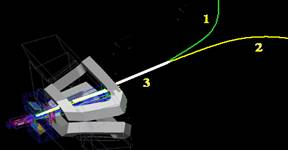
\includegraphics[width=0.5\textwidth]{ex_5_forca.jpg}
            \end{figure}
            \begin{enumerate}
                \item Sabendo-se que a carga elétrica da partícula 1 é positiva, qual a carga das outras duas partículas? Justifique.
                \item Qual o sentido do campo magnético? Justifique.
            \end{enumerate}
            
            \item \textbf{(UFMG-MG)} - Um feixe de elétrons passa inicialmente entre os pólos de um ímã e, a seguir, entre duas placas paralelas, carregadas com cargas de sinais contrários, dispostos conforme a figura a seguir. Na ausência do ímã e das placas, o feixe de elétrons atinge o ponto O do anteparo.
            \begin{figure}[h]
                \centering
                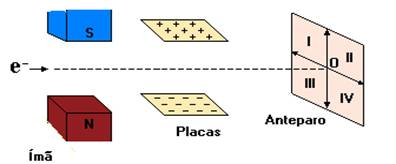
\includegraphics[width=0.5\textwidth]{ex_6_forca.jpg}
            \end{figure}
            
            Em virtude das opções dos campos magnético e elétrico, pode-se concluir que o feixe:
            \begin{enumerate}
                \item passará a atingir a região I do anteparo.
                \item passará a atingir a região II do anteparo.
                \item passará a atingir a região III do anteparo.
                \item passará a atingir a região IV do anteparo.
                \item passará a atingir a região O do anteparo.
            \end{enumerate}
            
            \item \textbf{(UFRGS - adaptado)} - No interior de um acelerador de partículas existe um campo magnético muito mais intenso que o campo magnético terrestre, orientado de tal maneira que um elétron lançado horizontalmente do sul para o norte, através do acelerador é desviado para o oeste. Para qual direção o campo magnético do acelerador aponta para?
            
            \item \textbf{(FGV-SP)} - Em 2008, o maior acelerador de partículas já construído foi colocado em funcionamento. Em seu primeiro teste, um feixe de prótons foi mantido em movimento circular dentro do grande anel, sendo gradativamente acelerado até a velocidade desejada.
            
            \begin{figure}[h]
                \centering
                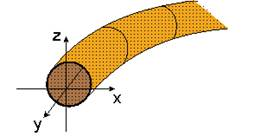
\includegraphics[width=0.5\textwidth]{ex_8_forca.jpg}
            \end{figure}
            
            A figura mostra uma secção reta desse anel. Admita que um feixe de prótons esteja sendo conduzido de modo acelerado no sentido do eixo y. De acordo com as leis do eletromagnetismo, os campos elétrico e magnético, nessa ordem, na origem do sistema de eixos indicado, têm sentidos que apontam para o:
            
            \begin{enumerate}
                \item positivo de y e negativo de z. 
                \item positivo de y e positivo de z. 
                \item positivo de y e positivo de x.
                \item negativo de y e positivo de z.  
                \item negativo de y e negativo de x.
            \end{enumerate}
            
            \item \textbf{(UFRRJ-RJ)} - Uma partícula de carga $q$ entra com velocidade $\vec{V}_o$ numa região onde existe um campo magnético uniforme $\vec{B}$. No caso em que $\vec{V}_o$ e $\vec{B}$ possuem a mesma direção, podemos afirmar que a partícula:
            
            \begin{enumerate}
                \item sofrerá um desvio para sua direita.
                \item sofrerá um desvio para sua esquerda.
                \item será acelerada na direção do campo magnético uniforme $\vec{B}$.
                \item não sentirá a ação do campo magnético uniforme $\vec{B}$.
                \item será desacelerada na direção do campo magnético uniforme $\vec{B}$.
            \end{enumerate}
            
            \item \textbf{(UFMG-MG)} - Em algumas moléculas, há uma assimetria na distribuição de cargas positivas e negativas, como representado, esquematicamente, na figura a seguir. 
            Considere que uma molécula desse tipo é colocada em uma região onde existem um campo elétrico ($\vec{E}$) e um campo magnético ($\vec{B}$), uniformes, constantes e mutuamente perpendiculares.
            
            Nas alternativas a seguir, estão indicados as direções e os sentidos desses campos. Assinale a alternativa em que está representada CORRETAMENTE a orientação de equilíbrio dessa molécula na presença dos dois campos.
            
            \begin{figure}[h]
                \centering
                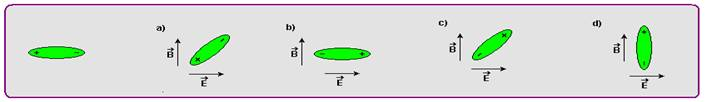
\includegraphics[width=0.9\textwidth]{ex_10_forca.jpg}
            \end{figure}
            
            \item \textbf{(UFJF-MG)} - Um filtro de velocidades é um dispositivo que utiliza campo elétrico uniforme ($\vec{E}$) perpendicular ao campo magnético uniforme ($\vec{B}$)  (campos cruzados), para selecionar partículas carregadas com determinadas velocidades. A figura a seguir mostra uma região do espaço em vácuo entre as placas planas e paralelas de um capacitor. Perpendicular ao campo produzido pelas placas, está o campo magnético uniforme. Uma partícula positiva de carga q move-se na direção z com velocidade constante (conforme a figura 1).
            
            \begin{figure}[h]
                \centering
                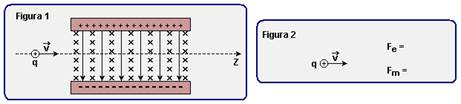
\includegraphics[width=0.8\textwidth]{ex_11a_forca.jpg}
            \end{figure}
            
            \begin{enumerate}
                \item Na figura 2, represente os vetores força elétrica,$\vec{F}_{el}$, e força magnética,$\vec{F}_{mag}$, que atuam na partícula assim que entra na região de campos cruzados, indicando suas magnitudes.
                \item Determine a velocidade que a partícula deve ter, para não ser desviada.
            \end{enumerate}
            
            \item \textbf{(Unimontes)} - Uma barra fina de cobre, de comprimento L = 0,5 m e massa m = 100 g, está inicialmente suspensa por dois fios de massa desprezível. A barra está imersa em campo magnético uniforme e de intensidade B = 10 T, cuja orientação é perpendicular e entrando no plano da folha. A gravidade no local possui módulo $g = 10 m/s^2$. Para anular a tensão nos fios que suportam a barra de cobre, é necessário que uma corrente I seja aplicada no sentido indicado na figura abaixo. O valor da corrente I, em ampères, deve ser:
            
            \pagebreak
            \begin{figure}[h]
                \centering
                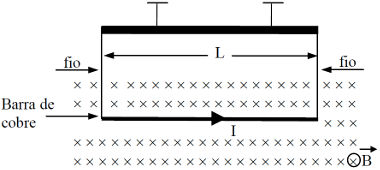
\includegraphics[width=0.4\textwidth]{ex_12_forca.jpg}
            \end{figure}
            
            \begin{enumerate}
                \item 0,2
                \item 0,4
                \item 0,3
                \item 0,5
                \item 0,7
            \end{enumerate}
            
            \item \textbf{(MACKENZIE-SP)} - Um condutor retilíneo de comprimento 0,5 m é percorrido por uma corrente de intensidade 4,0 A. O condutor está totalmente imerso num campo magnético de intensidade 10-3 T, formando com a direção do campo um ângulo de $30^{\circ}$. A intensidade da força magnética que atua sobre o condutor é de?
            
            \item \textbf{(UFRGS)} - Na figura a seguir, um fio condutor flexível encontra-se na presença de um campo magnético constante e uniforme perpendicular ao plano da página. Na ausência de corrente elétrica, o fio permanece na posição B. Quando o fio é percorrido por certa corrente elétrica estacionária, ele assume a posição A.
            \begin{figure}[h]
                \centering
                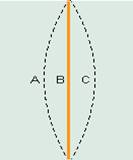
\includegraphics[width=0.4\textwidth]{ex_14_forca.jpg}
            \end{figure}
            
            Para que o fio assuma a posição C, é necessário
            \begin{enumerate}
                \item inverter o sentido da corrente e do campo aplicado.
                \item inverter o sentido da corrente ou inverter o sentido do campo.
                \item desligar lentamente o campo.
                \item desligar lentamente a corrente.
                \item desligar lentamente o campo e a corrente.
            \end{enumerate}
            
            \item \textbf{(UE-PB)} - Um professor de física resolve fazer um experimento de eletromagnetismo que objetiva determinar o valor do campo magnético entre os pólos do imã. Para isso, ele utiliza um imã, uma bateria que fornece 4,8V a um condutor cilíndrico AC com massa 5g, comprimento de 10cm e resistência elétrica igual a 0,10$\Omega$. Ao ligar a bateria ao circuito, mostrado na figura, o condutor cilíndrico fica suspenso em equilíbrio.
            
            \begin{figure}[h]
                \centering
                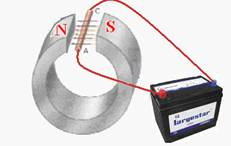
\includegraphics[width=0.5\textwidth]{ex_15_forca.jpg}
            \end{figure}
            Considerando-se que as linhas de campo são perpendiculares ao condutor, que a resistência elétrica dos fios é 0,02$\Omega$, que a massa dos fios é desprezível e adotando $g=10m/s^2$, o professor concluiu que o campo magnético, em Tesla, tem valor igual a:
            \begin{enumerate}
                \item $12,5*10^{-3}$
                \item $125$
                \item $1,25*10^{-4}$
                \item $12,5*10^{-2}$
                \item $1,25*10^{-2}$
            \end{enumerate}
            
            \item \textbf{(UFPE-PE)} - Um fio MN, de 40cm de comprimento e massa igual a 30g, está suspenso horizontalmente por uma mola ideal de constante elástica $k=10 N/m$. O conjunto encontra-se em uma região de campo magnético uniforme $B=0,1 Wb/m^2$, como mostra a figura.
            \pagebreak
            \begin{figure}[h]
                \centering
                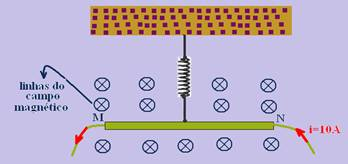
\includegraphics[width=0.5\textwidth]{ex_16_forca.jpg}
            \end{figure}
            
            Quando a corrente no fio for 10 A, dirigida de N para M, atuará sobre o fio uma força magnética verticalmente para baixo. Determine a elongação total, devido à força magnética e à força gravitacional, sofrida pela mola, em cm.
            
            \item \textbf{(UNICAMP-SP)} - Um fio condutor rígido de 200 g e 20 cm de comprimento é ligado ao restante do circuito por meio de contatos deslizantes sem atrito, como mostra a figura.
            
            \begin{figure}[h]
                \centering
                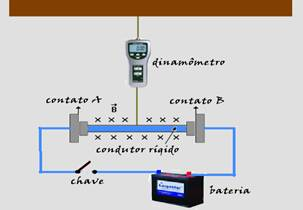
\includegraphics[width=0.5\textwidth]{ex_17_forca.jpg}
            \end{figure}
            
             O plano da figura é vertical. Inicialmente a chave está aberta. O fio condutor é preso a um dinamômetro e se encontra numa região com campo magnético de 1,0T, entrando perpendicularmente no plano da figura: (\textit{Obs: Considere $g=10m/s^2$})
             
             \begin{enumerate}
                 \item Calcule a força medida pelo dinamômetro com a chave aberta, estando o fio em equilíbrio.
                 \item Determine a direção e a intensidade da corrente elétrica no circuito após o fechamento da chave, sabendo-se que o dinamômetro passa a indicar leitura zero.
                 \item Calcule a tensão da bateria sabendo-se que a resistência total do circuito é de $6,0\Omega$.
             \end{enumerate}
             
             {\large \textbf{As questões 18 e 19 tratarão a seguinte imagem e o seguinte enunciado:}}
             
             A figura abaixo mostra uma região onde existe um campo magnético uniforme, de módulo igual a $5,0*10^{-1}\: T$, localizado entre os pólos de um imã. Nessa região, há uma mola ideal , de constante elástica k igual a $2,0*10^2\: N/m$, presa ao teto, que sustenta em sua extremidade um fio cilíndrico, condutor e retilíneo, de comprimento L igual a 2,0m e massa M igual a $6,0*10^2\:g$. O fio é percorrido por uma corrente contínua i, cujo sentido está indicado pelo símbolo $\otimes$.
             \begin{figure}[h]
                 \centering
                 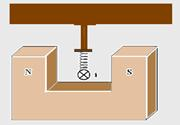
\includegraphics[width=0.5\textwidth]{ex_18_19_forca.jpg}
             \end{figure}
             
             \item \textbf{(IFET-MG)} - Observando a figura acima, podemos concluir que a força magnética que atua sobre o fio apontará: 
             
             \begin{enumerate}
                 \item verticalmente para baixo.
                 \item verticalmente para cima.
                 \item perpendicularmente ao plano do papel, afastando-se do leitor. 
                 \item perpendicularmente ao plano do papel, aproximando-se do leitor. 
                 \item horizontalmente para a direita.
             \end{enumerate}
             
             \item \textbf{(IFET-MG)} -Admitindo que o sistema esteja em equilíbrio e adotando a aceleração da gravidade  g igual a $10\: m/s^2$, o valor da deformação x sofrida pela mola quando a corrente i for igual a $4,0*10^{-1}\: A$ é, em módulo, igual a:
             
             \begin{enumerate}
                 \item $32 \: cm$
                 \item $64\: cm$
                 \item $6,4*10^{-2} \: m$
                 \item $3,2*10^{-2}\: m$
                 \item $3,2*10^{-2}\: cm$
             \end{enumerate}
        \end{enumerate}
        
    \end{itemize}
    
    \pagebreak
    \section*{GABARITO}
    \begin{itemize}
        \item \textbf{Campo Magnético}
        \begin{enumerate}
            \item (e)
            \item 1000
            \item (b). O item (a) está errado porque o campo é proporcional ao número de espiras. O item (c) está errado, pois as linhas de campo do solenóide são paralelas ao solenóide. O item (d) está errado, pelo motivo dado ao item (c).
            \item (a)
            \item (a)
            \item (b) 
            \item 
            \begin{enumerate}
                \item Como a circunferência inteira tem resistência igual a $8 \Omega$, então o trecho AB, que é um 1/4 de circunferência, tem resistência: $R_1 = 8*1/4 = 2 \Omega$. E o do restante do trecho, que é 3/4 da circunferência: $R_2 = 8* 3/4 = 6 \Omega$.
                
                Há 2 caminhos possíveis para de ir A a B: por $R_1$ e por $R_2$. Então, usando a Lei de Ohm: $U = R_1*i_1$ e $U = R_2*i_2$. 
                Colocando os valores e igualando ambas equações: $2*i_1 = 6*i_2$ (eq.1).
                
                Em A, há uma bifurcação, então usamos a conservação de corrente: $i_1 + i_2 = 4$ (eq.2)
                
                Agora temos um sistema de equações e podemos descobrir as correntes. Isolando $i_1$ na (eq.1) e substituindo na (eq.2): $3*i_2 + i_2 = 4 \implies i_2 = 1$A.
                
                Substituindo $i_2$ de volta na (eq.1): $2*i_1 = 6 \implies i_1 =3$A.
                
                \item Pela Regra da Mão Direita, cada corrente vai gerar um campo magnético ($\vec{B}_1$ e $\vec{B}_2$) em direções opostas. 
                
                Como a parte de $i_1$ só percorre 1/4 da circunferência, o campo magnético no centro é: $B_1 = 1/4 * \frac{\mu*i_1}{2R} \implies B_1 = \frac{3\mu}{8R}$.
                
                Como a parte $i_2$ percorre o 3/4 da circunferência, o campo magnético no centro é: $B_2 = 3/4 * \frac{\mu * i_2}{2R} \implies B_2 = \frac{3\mu}{8R}$.
                
                Como o campo magnético total é: $B= B_1 + B_2$ e ambos tem o mesmo valor, só que direções opostos, $B_1$ e $B_2$ se anulam, logo $B = 0$ no centro.
                \end{enumerate}
            \item $\frac{i_1}{i_2} = 0,4$
            \item (c)
            \item (a)
            \item \begin{enumerate}
                \item Perpendicular á folha, saindo dela.
                \item $\frac{i_2}{i_1} = 3$
            \end{enumerate}
            \item (c)
            \item (e)
            \item (a)
        \end{enumerate}
        
        \item \textbf{Força Magnética}
        
        \begin{enumerate}
            \item (a)
            \item (c)
            \item (a)
            \item (a)
            \item 
            \begin{enumerate}
                \item Carga 2 - negativa, carga 3 - neutra, porque a direção da força magnética sobre negativa é oposta a da força sobre carga positiva e força magnética só age sobre uma carga elétrica, logo algo neutro não é afetado.
                \item Como a carga 1, que é positiva, faz uma curva para esquerda, a força magnética é para a esquerda. Dado que a carga 1 tem velocidade para frente inicialmente, pela Regra da Mão Esquerda, o campo magnético sai pela folha ( $\odot$).
            \end{enumerate}
            \item (a)
            \item Orientando o Norte-Sul verticamente, igualmente a uma bússola, a direção do campo magnético do acelerador é saindo da folha ( $\odot$). (\textit{Obs: lembra que o elétron é uma carga negativa, logo tem que inverter a direção obtida a partir da Regra da Mão Esquerda})
            \item (a)
            \item (d)
            \item (b) (\textit{Obs: aqui, equiíbrio significa que a molécula está parada. Ou seja, não há movimento.}
            \item \begin{enumerate}
                \item A força elétrica ($\vec{F}_{el}$) aponta para baixo e a força magnética ($\vec{F}_{mag}$), pela Regra da Mão Esquerda, aponta para cima.
                \item Para não ser desviada, as forças elétrica e magnética devem se anular. Portanto:
                \begin{align*}
                    F_{el}&=F_{mag} \\
                    q.E &= q.V.B \implies V = \frac{E}{B}
                \end{align*}
            \end{enumerate}
            \item (a)
            \item $2*10^{-2}$ N
            \item (b)
            \item (e)
            \item $x=7,0\: cm$ (\textit{Obs: $Wb/m^2 = T$})
            \item \begin{enumerate}
                \item $T=2,0\:N$ 
                \item Corrente tem que ter direção horizontal com sentido para direita.
                \item $U=60\:V$
            \end{enumerate}
            \item (a)
            \item (d)
        \end{enumerate}
    \end{itemize}
\end{document}
